% !TEX root = ./main.tex
% !TEX encoding = UTF-8 Unicode
% !TEX program = pdflatex
% !TeX spellcheck = it_IT

\graphicspath{{Immagini/},{Immagini/android_aging/}}

\chapter{Software Aging on Android 7}

\section{Traccia}
Verificare se \textbf{Android} è soggetto ad \textbf{\textit{aging}}.\\

\section{System Under Test}
Il disposito utilizzato è un \textbf{Huawei P9 Lite}, con le seguenti caratteristiche:

\begin{itemize}
  \item \textbf{Chipset: }Kirin 650 (4 x 2,0GHz + 4 x 1,7GHZ) 64 bit
  \item \textbf{Memoria: } 3GB RAM, 16GB EMMC Flash ROM
  \item \textbf{Sistema Operativo: }Android 7.0
\end{itemize}

\section{Experimental plan}

Per verificare il fenomeno dell'\textbf{Aging} sarà analizzato il \textbf{Lunch Time(LT)},
il quale misura il tempo tra il click sull'icona dell'applicazione e l'avvio della stessa,
in quanto il fenomeno dell'invecchiamento, dal punto di vista dell'utente, è visto come la
non reattività del dispositivo.\\
Gli indicatori di aging di sistema sono invece parametri che riguardano la memeoria,
\textit{Garbage Collection} e \textit{Task-Level}.\\

\section{Experimental Setup}

Gli esperimenti sono stati eseguiti su di un \textit{Huawei P9 Lite}, descritto
precedentemente, utilizzando il tools \textit{\textbf{ADB(Android Device Bridge)}}.\\
La generazione del workload è stata effettuate tramite il tools
\textit{\textbf{Monkey WL generator}}, mentre la raccolta dei dati è stata
effettuata tramite le utility \textit{\textbf{dumpsys}} e \textit{\textbf{logcat}}.
In figura \ref{setup} è riportato lo schema di connessione con il quale sono stati
eseguiti gli esprimenti.\\
La connessione tra pc ed smartphone è stata effettuate tramite WiFi, quindi è
stato generato il workload tramite \textit{\textbf{Monkey WL generator}} e inviato
tramite WiFi al dispositivo mobile,  successivamente i dati sono stati raccolti
utilizzando  \textit{\textbf{dumpsys}} e \textit{\textbf{logcat}}.

\begin{figure}[!htbp]
  \centering
  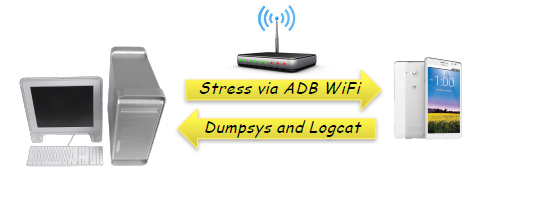
\includegraphics[width=\linewidth, keepaspectratio]{setup}
  \caption{Setup esperimenti}
  \label{setup}
\end{figure}

Sono stati eseguiti due test il primo a workload fisso mentre in secondo a workload
variabile.\\
Il primo esperimento è un test che punta a stressare il dispositivo effettuando
un'operazione ogni 100 ms, la durata di tale test è di 6 ore.
Il secondo esperimento è un test che punta ad osservare il comportamento del dispositivo
in utilizzo normale, come se fosse un classico utente ad utilizzarlo, quindi effettua
delle operazioni ad intervallo di tempo variabile(500 ms, 1500 ms e 2500 ms), quindi la durata di tale test è di
12 ore.\\
In particolare il workload genera i seguenti movimenti
\begin{itemize}
  \item Touch, Motion and Trackballs (33\%);
  \item (minor and major) Navigation (33\%);
  \item AppSwitch (34\%).
\end{itemize}
Le applicazioni lanciate negli esperimenti sono riportate nella tabella in figura
\ref{applicazioni}, ottenute lanciando il comando \textit{adb shell pm list
packages}.\\

\begin{figure}[!htbp]
  \centering
  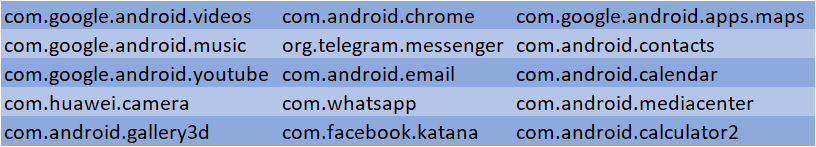
\includegraphics[width=\linewidth, keepaspectratio]{applicazioni}
  \caption{Applicazioni Workload}
  \label{applicazioni}
\end{figure}

L'esecuzione degli esperimente è stata effettua lanciando lo script bash
\textit{\textbf{runtest.sh}} il quale richiama i seguenti script:
  \begin{itemize}
    \item \textit{\textbf{logcat\_art.sh}}: raccoglie i dati relativi al \textit{Garbage Collector};
    \item \textit{\textbf{dumpTask.sh}}: raccoglie i dati relativi ai task;
    \item \textit{\textbf{dumpOnlyMeminfo.sh}}: raccoglie i dati relativi alla memoria;
    \item \textit{\textbf{loagcat\_displayed.sh}}: raccoglie i dati relativi al LT;
    \item \textit{\textbf{kill\_after\_time.sh}}: permette di definire il tempo di
    sperimentazione ed esegue il reboot in modalità recovery del dispositivo;
    \item \textit{\textbf{LaunchTimeMeasurement.sh}}: esegue lo stess test del dispositivo;
    \item \textit{\textbf{WorkloadFixed.sh o WorkloadVariable.sh}}: il primo definisce le applicazioni del
    workload fisso, il secondo definisce l'esecuzione del workload variabile richiamando
    ulteriori 3 script nel quale sono definite le applicazioni da lanciare.
  \end{itemize}

\section{Data Analisys}

L'esecuzione dello script \textbf{\textit{runtest.sh}} genera diversi file di log
tra cui \textit{\textbf{Displyed.txt}} e \textit{\textbf{meminfo.txt}} i quali
contengono rispettivamente i dati relativi ai tempi di lancio delle activity e
i dati relativi all'utilizzo della memoria.\\
L'analisi relativa ai tempi di lancio è effettuata tramite lo script \textbf{\textit{generate\_Time\_data.sh}},
il quale estrae una serie temporale per ogni activity, sulle quali effettua
tramite un script R il \textbf{\textit{Mann Kendall test}} con intervallo
di confidenza al 90\%.\\
Il \textbf{\textit{Mann Kendall test}} è un test che mira a verificare l'esistenza
di un trend, infatti l'ipotesi nulla di tele test è l'esistenza di un trend quindi
valori bassi del p-value rifiutano $H_0$.\\
Inoltre lo script genera i plot per ogni activity.\\
L'analisi relativa alla memoria è effettuata tramite gli script:
\begin{itemize}
  \item \textit{\textbf{generate\_Meminfo\_data.sh}}:
  \item \textit{\textbf{generate\_Global\_Meminfo\_data.sh}}: genera le statistiche
  globali per i parametri di memoria RAM e i relativi plot temporali;
  \item \textit{\textbf{generate\_Meminfo\_data\_Slopes.sh}}: esegue il \textbf{\textit{Mann Kendal test}}
  per ogni task attivo sul dispositivo;
\end{itemize}

\subsubsection{Launch Time Analisys(Worklaod Fixed)}
Dopo aver analizzato il valori di \textit{slop}(pendenza della retta) e
\textit{p-value}(relativo al Mann Kendall test) 
\subsubsection{Launch Analisys(Worklaod Variable)}

\subsubsection{Memory Time Analisys(Worklaod Fixed)}

\subsubsection{Memory Time Analisys(Worklaod Variable)}
